\section{\Shadow{}}
\label{s:algo}
\Scrooge{} aims to efficiently implement the \CCC{} primitive without relying 
on any trusted third-party code or infrastructure and without broadcasting 
multiple copies of a message across the network.
%Prior works attempt to implement the \CCC{} primitive in following ways:
%(1) deploying trusted hardware and infrastructure,
%(2) employing zero knowledge proofs, and
%(3) concurrently sending multiple copies of each message.
%The key challenge with the use of trusted hardware is that they 
%are expected to remain honest, which makes them a sink for all attacks.
%Solutions based on zero knowledge proofs 
%are not only computationally expensive to generate, but also  and have high latencies.
%
%Alternatively, each \RSM{} can create and send multiple copies of each message, 
%but this design requires deciding which replica(s) in the \RSM{} will send the message to 
%which replica(s) in the receiver \RSM{}.
%Some \RSM{}-to-\RSM{} communication protocols opt for the hands-off {\em all-to-all} communication 
%where every replica in the sending \RSM{} sends a copy of the message to every replica in the receiving \RSM{}.
%Other protocols attempt to communicate only linear number of messages, but they 
%fall back to the all-to-all communication for recovery from Byzantine attacks.
%Moreover, these solutions expect a synchronous network.
\Scrooge{} offers the following appealing properties:
\begin{enumerate}[wide,nosep,label=(P\arabic*),ref={P\arabic*}]
\item \label{g:hetero} {\bf Heterogeneity.}
\Scrooge{} facilitates communication between two \RSM{s} with arbitrary sizes and failure models.

\item \label{g:async} {\bf Asynchrony.}
\Scrooge{} does not require a synchronous network to reliably deliver messages across \RSM{s}.

\item \label{g:single} {\bf Singularity.}
\Scrooge{} saves available bandwidth by creating zero copies of each message in the good case.

\item \label{g:recovery} {\bf Optimal Recovery.}
\Scrooge{} introduces constant-sized cumulative \quack{s} to detect and recover from failures.

\item \label{g:bidrect} {\bf Duality.}
\Scrooge{} allows both \RSM{s} to simultaneously send and receive messages;
\Scrooge{} harnesses this bi-directional pattern to piggyback acknowledgments.

\item \label{g:indepen} {\bf Independence.}
\Scrooge{} prevent an honest sender/receiver to be forever stuck with a Byzantine 
sender/receiver.

\end{enumerate}

\begin{figure}[t]
    %\vspace{-6mm}
    \centering
    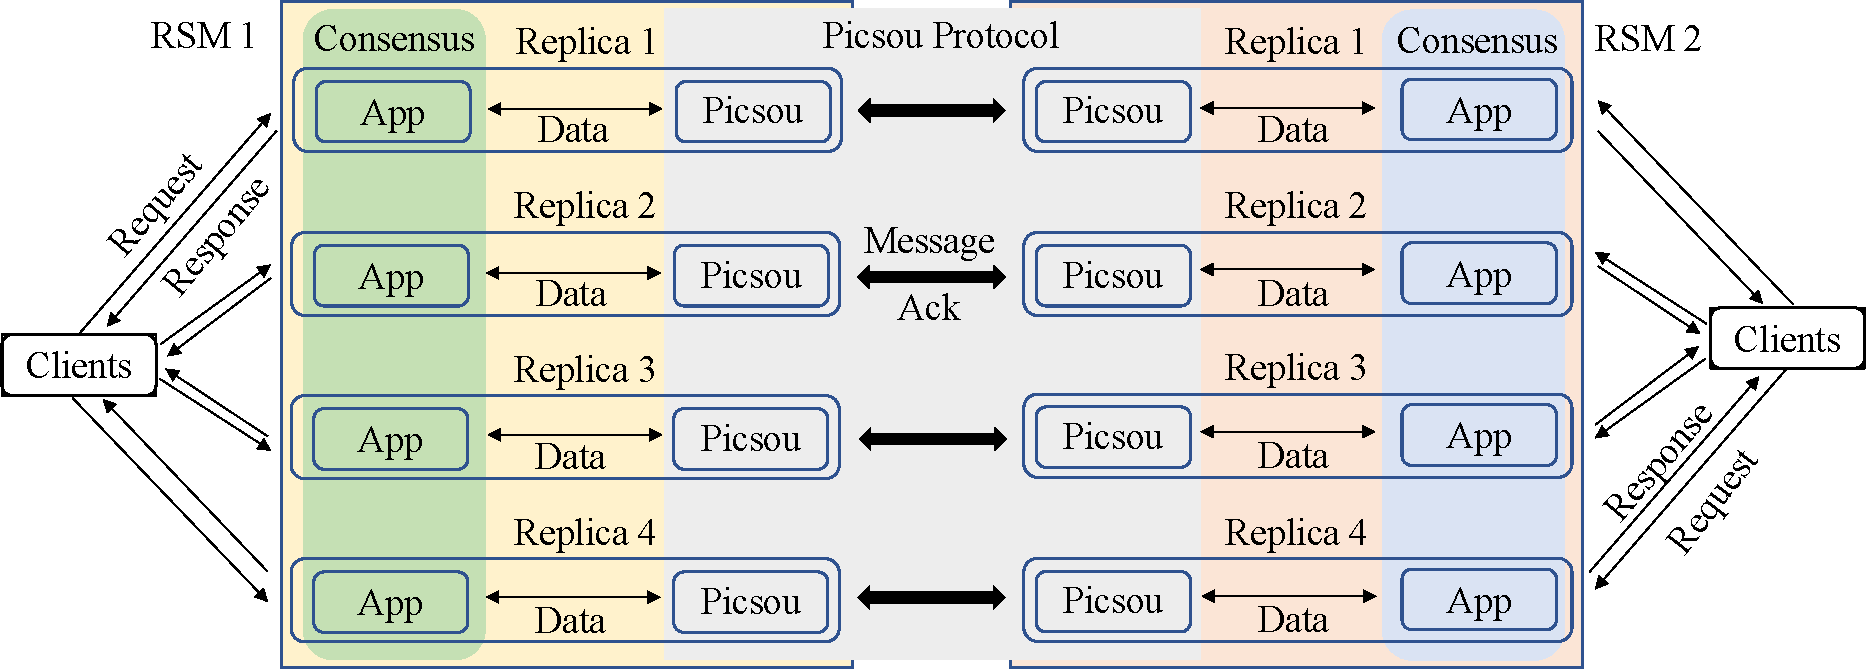
\includegraphics[width=0.85\columnwidth]{end-flow.pdf}
    %\vspace{-2mm}
    \caption{An illustration of \CCC{} primitive between two \RSM{s}, which employ some consensus protocol to manage their states and
    adopt \Scrooge{} for exchanging messages.}
    \label{fig:end-flow}
\end{figure}

In Figure~\ref{fig:end-flow}, we illustrate how \Scrooge{} implements \CCC{} primitive between two \RSM{s} 
and guarantees an end-to-end data flow that meets our aforementioned properties.
For the sake of understanding, in this section, we assume that all the replicas have equal shares.
Each \RSM{} receives requests from clients and runs its choice of consensus protocol to commit those requests. 
To do so, each replica runs an instance (App) of the consensus protocol.
Post this, each replica communicates the committed requests to the co-located \Scrooge{} instance, which 
follows the \Scrooge{} protocol to send the message to a replica in the other \RSM{}.
Once the sending \Scrooge{} instance receives a cumulative \quack{} for the sent message, 
it acknowledges the receipt of the message to the co-located consensus instance.
Similarly, when the receiver receives a valid message, it forwards that message to its corresponding consensus instance.

Internally, a sender \Scrooge{} instance does the following tasks:
(1) Randomly select a receiver.
(2) Determine message to send.
(3) Send the message.
(4) Piggyback cumulative acknowledgments for received messages.
(5) Collect \quack{s} for sent messages.
%
Similarly, a receiver \Scrooge{} instance does the following tasks:
(1) Validate the received message, if invalid, discard.
(2) Send cumulative acknowledgment to the sender.
(3) Broadcast the received message in its \RSM{}.
%
Notice that \Scrooge{} is oblivious to clients and disinterested in the content of the message.


{\bf Message Format.}
To meet the desired goals, every \Scrooge{} instance expects that the 
corresponding consensus instance only forwards {\em committed} requests;
a committed request is expected to accompany a {\em proof}, which illustrates that a quorum of 
replicas in this \RSM{} have ordered this request.
However, consensus instances running on Byzantine replicas may not fulfill this requirement, 
and in \S~\ref{s:fail} we present steps to overcome various failures.
We expect the following from each honest consensus instance:
(1) It forwards all the requests that need to be sent to the other \RSM{} to its co-located Scrooge instance. 
(2) It ensures that each forwarded request is of the form $\SignMessage{m, \Seqn}{\Qusign{i}}$, 
where $m$ is a request committed at sequence number $\Seqn$ by a quorum of replicas in \RSM{} $\SMR{i}$ 
and $\Qusign{i}$ includes the digital signatures of this quorum.


{\bf Destination and Message Discovery.}
Although each \Scrooge{} instance has access to all the committed requests, 
to meet the promise of zero copy transmission,
we ask each instance to send a {\em unique} committed request to the other \RSM{}.
This uniqueness also brings forth three key challenges:
(1) which request to send, 
(2) whom to send, and
(3) how to detect successful transmission.

We handle the first challenge by evenly dividing all the messages to be sent across all the 
\Scrooge{} instances.
To do so, we perform the $\bmod$ operation as follows: 
$\Seqn \bmod j$, where the message with sequence number $\Seqn$ is sent by $j$-th \Scrooge{} instance.
%
To meet the next two challenges, we need to determine the destination for each message. 
A naive way to do so would be to enable {\em static pairing} where each sender is paired 
with one receiver (replica at the other \RSM{}) and the sender sends all its messages to this one receiver.
There is a key limitation of static pairing: 
either the sender or the receiver may act Byzantine, which makes it impossible to determine if a message 
has been received at the destination \RSM{}.

As a result, our \Scrooge{} protocol dynamically switches pair using the round-robin protocol.
A $j$-th \Scrooge{} instance determines the identity of the next receiver by running the mod operation 
over the identifier of the previous receiver:
\begin{equation}
 \text{next receiver} =  (j + 1) \bmod \n{i}
\end{equation}
where $j$ is the identifier of the previous receiver and $\n{i}$ are the number of replicas in the receiving \RSM{}.
To ensure every instance starts with a different receiver, the first receiver for the $j$-th 
instance is the replica with identifier $j$.

Next, we illustrate the three step \Scrooge{} protocol.
For simplicity, we will assume that replicas in \RSM{} $\SMR{1}$ (sender \RSM{}) 
want to communicate messages to replicas in \RSM{} $\SMR{2}$ (receiver \RSM{});
this protocol can be used to send messages in either directions.
Further, we assume that all the committed requests received by \Scrooge{} instances 
have continuous sequence numbers;
in \S~\ref{ss:cum-quack}, we show how to trivially eliminate this requirement.


\subsection{Message Transmission}
\label{ss:transmit}
When the $j$-th replica $\Replica{1}{j}$ of \RSM{} $\SMR{1}$ receives a committed request
$\SignMessage{m}{\Qusign{1}}$ from the co-located consensus instance, 
it determines if it is responsible for sending this message. 
To do this, $\Replica{1}{j}$ takes the sequence number of this request (say $\Seqn$) 
and runs the $\bmod$ operation.
If this is the case, $\Replica{1}{j}$ determines the receiver for this message using 
the destination discovery procedure described earlier. 
Assume replica $\Replica{2}{l}$ of the \RSM{} $\SMR{2}$ is the intended receiver.
Finally, $\Replica{1}{j}$ creates a message $\SignMessage{m, \Seqn}{\Qusign{1}}$ and 
sends this message to $\Replica{2}{l}$.

Note: 
(1) $\Replica{1}{j}$ uses \Name{Mac} to sign the message $\SignMessage{m, \Seqn}{\Qusign{1}}$ 
prior to sending it to $\Replica{2}{l}$; this $\Name{Mac}$ prevents an adversary from 
intercepting the message and modifying its content.
(2) Each message is sent by only one replica of \RSM{} $\SMR{1}$, thereby, 
zero copy transmission.


\subsection{Message Reception}
When the $l$-th replica $\Replica{2}{l}$ receives a message $\SignMessage{m, \Seqn}{\Qusign{1}}$ 
from a replica in \RSM{} $\SMR{1}$, it checks if $\Qusign{1}$ includes signatures of a 
quorum of replicas of \RSM{} $\SMR{1}$ for message $m$. 
If this is the case, $\Replica{2}{l}$ assumes that $m$ is a valid request committed 
at sequence number $\Seqn$ and sends an acknowledgment to replica $\Replica{1}{l}$.
Finally, replica $\Replica{2}{l}$ {\em broadcasts} this message $\SignMessage{m, \Seqn}{\Qusign{1}}$ in its \RSM{};
broadcast helps other replicas in the \RSM{} to receive the message and acknowledge 
its receipt in the future.

Note: 
if the receiver $\Replica{2}{l}$ also has some message (any committed request that it 
received from its \RSM $\SMR{2}$) 
to send to replica $\Replica{1}{j}$,
it can simply piggyback the acknowledgment message with this message.


\subsection{Cumulative Quorum Acknowledgment}
\label{ss:cum-quack}
The key ingredient behind \Scrooge's aforementioned six appealing properties is its 
cumulative quorum acknowledgments (\quack{}).
Cumulative \quack{s} are constant-sized and help all the sending \RSM{}
replicas determine 
whether at least one honest party at the receiving \RSM{} received the message.
\Scrooge{} provides all the sending \RSM{} replicas (not only the sender)  
acknowledgments for each message sent so that they can detect any failures.

Without cumulative \quack{s}, for each message sent, each sending \RSM{} replica 
would require acknowledgments from a quorum of replicas of the receiving \RSM{}.
As up to $\f{2}$ replicas of the receiving \RSM{} can act Byzantine, the quorum size  
is $\f{2}+1$, which proves that at least one honest party received the message.
Clearly, sending $\f{2}+1$ acknowledgments per message will exhaust the available bandwidth.

\Scrooge{} aggregates multiple acknowledgments together and 
sends a single cumulative acknowledgement.
Specifically, each receiver maintains a contiguous set of messages $\SAck{}$.
Prior to receiving any message, each receiver initializes its set $\SAck{}$ with a {\em null} element ($\phi$).
Whenever a replica receives a message $m$ with sequence number $\Seqn$ from the sending \RSM{}, 
it adds it to the set $\SAck{}$
if $\Seqn$ is one more than the largest sequence number in $\SAck{}$; the first addition to $\SAck{}$ is message 
with $\Seqn = 0$.
Otherwise, it holds adding the message with higher sequence number until the messages with lower
sequence number arrives.

Post this, the receiver finds the last sequence number (also the highest) in the set $\SAck{}$ (say $\Seqn$)
and sends a message $\Ack{\Seqn}$ to the sender.
Notice that initially, receivers send message $\Ack{\phi}$ until they have access to a message with sequence number $\Seqn=0$.
Once it receives the message with $\Seqn=0$, for any messages it receives in the future, 
it sends an acknowledgment $\Ack{p}$, if $\SAck{}$ includes all the messages between $\Seqn=0$ and $\Seqn=p$.
%
%For example, assume replica $\Replica{2}{l}$ has already acknowledged message $\SignMessage{m,5}{\Qusign{1}}$
%and is yet to acknowledge messages $\SignMessage{m,6}{\Qusign{1}}$ and $\SignMessage{m,7}{\Qusign{1}}$ 
%when it receives message $\SignMessage{m,8}{\Qusign{1}}$ from replica $\Replica{1}{j}$.
%Hence, it creates a cumulative acknowledgment $\Ack{8}$ and sends it to $\Replica{1}{j}$.
%
Thus, when the sender receives a cumulative acknowledgment (say $\Ack{p}$), it determines
that messages up to sequence number $p$ have been received by at least one replica in the receiving \RSM{}.
When does this sender marks the message with sequence number $\Seqn$ 
received by at least one honest replica in the receiving \RSM{}? 
When it receives cumulative acknowledgements for messages with sequence number $\ge p$
from at least $\f{2}+1$ distinct receivers.
This set of $\f{2}+1$ acknowledgments for a message $m$ is what we term as a \quack{} for $m$.

%Note: although each replica sends each message to only one receiver, 
%it is able to create a \quack{} as it runs our round robin algorithm to determine the destination for each message.
%Consequently, each replica ends up sending some message to each replica in the other \RSM{}.



\section{Weighted \RSM{s} -- Stakes}
\label{s:stake}
Until now, we assumed that all the replicas have equal shares or stakes. 
However, several existing systems allow replicas to have different shares, 
where a replicas' share determines its decision making power in the \RSM{}.
This brings forth several new challenges for our \Scrooge{} protocol.
\begin{enumerate}
    \item For each \RSM{}, the notations $\n{}$ and $\f{}$ refer to the total 
    stake and Byzantine stake and not the traditional terminology for referring to 
    number of replicas.
    This implies that the total $\n{}$ stake is distributed among less than $\n{}$ replicas.

    \item Each sender with stake $> 1$ would have to send multiple consecutive messages 
    to one receiver.
    As a result, the acknowledgments from the receiving \RSM{} will also be proportional 
    to the stake of the receiver.

\end{enumerate}

To allow our \Scrooge{} protocol to handle such weighted \RSM{}, we need to modify 
the way a sender discovers messages to send, intended receiver, and counting cumulative \quack{}.

\begin{figure}[t]
    \begin{myprotocol}
	\INITIAL{Initialization:}{\newline
	{%\color{orange}
	// $\SMR{1} :=$ \RSM{} of the replica calling this function.\newline
	// $\SMR{j} :=$ Receiver \RSM{}.
	}}
	\vspace{1mm}

	\FUNC{sws}{message identifier: $\Seqn$; sorted List: $\SList$}
		\STATE $\DList$ $:=$ $\SList$ (Temporary list).
            \STATE $\n{j}$ $:=$ Total stake of $\SMR{j}$.
            \STATE $orig$ $:=$ $\Seqn \bmod \n{j}$
            \STATE $iter$ $:=$ $\lfloor \Seqn / \n{j} \rfloor$
            \STATE $dest$ $:=$ $(orig + iter) \bmod \n{j}$.
		\STATE {\bf return} $dest$.
	\ENDFUNC
	\SPACE
    \end{myprotocol}
    \caption{Sharewise Scheduler to identify the message receivers.}
    \label{func:sws}
\end{figure}



{\bf Dynamic Sharewise Scheduler.}
First, we modify the protocol for selecting the destination for a message. 
We can no longer use the round robin protocol $+$ $\bmod$ operation (\S~\ref{s:algo}) 
as it is oblivious to the total shares of each \RSM{} and the shares of each replica and 
sends all the replicas in the receiving \RSM{} an equal number of messages.
This in turn would send more messages to Byzantine receivers, which can deteriorate the 
performance of the \Scrooge{} protocol.

To this end, we design a Dynamic Sharewise Scheduler (\SWS), which builds on top of the 
Completely Fair Scheduler (\CFS{})~\cite{cfs} algorithm.
Prior to running the \SWS{} scheduler, we normalize the total shares of each \RSM{}. 
with their {\em least common multiple} (LCM). 
For example, assume $\n{1}$ and $\n{2}$ are the total shares of \RSM{} $\SMR{1}$ and $\SMR{2}$, 
and $\n{1}\times\n{2}$ is the LCM, then normalizing the shares requires multiplying 
the shares of each replica in $\SMR{1}$ with $\n{2}$ and the shares of each replica in $\SMR{2}$ with $\n{1}$.
%As we will see below, this normalization eases the mapping between replicas of $\SMR{1}$ and $\SMR{2}$.

Next, each sender calls the \SWS{} protocol (Figure~\ref{func:sws})
with the sequence number of the message ($\Seqn$) as input.
The \SWS{} protocols returns $dest$ as output, which states the ``share''
responsible for receiving this message.
Finally, the sender translates the $dest$ share to the identity of corresponding receiver replica, 
which is a trivial task given the knowledge of shares and identifiers of all replicas.
Instead of returning the identifier of the replica, \SWS{} returns the responsible 
share because the protocol views the total share $\n{j}$ of an \RSM{} $\SMR{j}$ as $\n{j}$ distinct identities.


\subsection{Weighted \Scrooge{}}
With weighted \RSM{s}, we need to slightly modify our basic \Scrooge{} protocol.
The {\em message transmission} step remains unchanged except that each sender calls the dynamic \SWS{} scheduler  
to identify the receiver for a message. 
As earlier, for deciding if a replica with identifier $l$ and share $\share{j}$ 
of the \RSM{} $\SMR{i}$ is responsible for sending the message with sequence number $\Seqn$, 
we perform the operation $\Seqn \bmod \n{i}$.
However, instead of providing the identifier for a replica, each sender receives the information about 
the responsible share, which is trivial to map to the sender identifier.

Similarly, {\em message reception} step remains unchanged.
However, there is a small change in the way a sender reaches a cumulative \quack{}. 
In the basic \Scrooge{} protocol, the sender waits for cumulative acknowledgment 
messages for message $m$ from $\f{2}+1$ distinct replicas of the receiving \RSM{} $\SMR{2}$ 
before concluding that $m$ has been successfully received by at least one honest 
replica of $\SMR{2}$.
This principle may not apply when the \RSM{s} are weighted because the total number of 
distinct replicas are no longer bounded by notations $\n{}$ and $\f{}$. 
Thus, each cumulative acknowledgment message is now weighted; 
acknowledgment message from a $l$-th replica with share $\share{l}$ has a weight $\share{l}$.
As a result, the sender marks a message $m$ received at \RSM{} $\SMR{j}$ when 
the total weight of cumulative \quack{} for $m$ from $\SMR{j}$ is equal to $\f{j}$.




%\item {\bf Transmit.}
%On calling the function \SWS{}, each replica $\Replica{i}{l}$ receives a list of replicas ($\DList$) it needs 
%to send messages.
%\Scrooge{} requires $\Replica{i}{l}$ to send each replica in $\DList$ a unique message from its $\Sbuf{l}$.
%To determine which messages from $\Replica{i}{l} $ each replica in $\DList$ receives, $\Replica{i}{l}$ calls the function 
%{\bf transmit} in Figure~\ref{func:sws}.
%In this function, we use the extracted messages to refer to messages with the least sequence number.
%
%\begin{example}
%Say the call to function $\SWS{}$ by replica $\Replica{i}{l}$ with share $\share{l} = 3$ returned 
%$\DList{} = \{\Replica{j}{r}, \Replica{j}{s} \}$, such that $\share{r} = 2$ and $\share{s} = 3$.
%Assume 
%\[\Sbuf{l} = \{ \SignMessage{m,k}{\Qusign{i}}, \SignMessage{m',k'}{\Qusign{i}}, \SignMessage{m^\circ,k^\circ}{\Qusign{i}}, \SignMessage{m^{\star},k^{\star}}{\Qusign{i}},... \}\]
%such that $k < k' < k^\circ < k^\star$.
%After sending every three messages from $\Sbuf{l}$, $\Replica{i}{l}$ loops back to $\DList$.
%Specifically, $\Replica{i}{l}$ extracts $\SignMessage{m,k}{\Qusign{i}}$ and $\SignMessage{m',k'}{\Qusign{i}}$ and sends to $\Replica{j}{r}$, 
%extracts $\SignMessage{m^\circ,k^\circ}{\Qusign{i}}$ and sends to $\Replica{j}{s}$, and cycles back to $\Replica{j}{r}$
%and sends it $\SignMessage{m^{\star},k^{\star}}{\Qusign{i}}$.
%As a result, in each cycle $\Replica{i}{l}$ sends $\Replica{j}{s}$ only one message even though $\share{s} = 3$.
%
%\end{example}

%\item {\bf Cumulative Acknowledgments.}
%If the two \RSM{s} are participating in bidirectional communication streams,  
%it is possible that $\Replica{i}{l}$ may have received messages from some replicas in \RSM{} $\SMR{j}$.
%We require $\Replica{i}{l}$ to acknowledge each message it received from \RSM{} $\SMR{j}$. 
%To conserve bandwidth, instead of sending an acknowledgment for each received message, 
%\Scrooge{} requires $\Replica{i}{l}$ to create cumulative acknowledgments and {\em piggyback} them with 
%the outgoing messages.
%
%Prior to sending a message,
%each replica searches its list $\SAck{l}$ for the longest contiguous set of acknowledgments.
%The last acknowledgment of this contiguous list is considered as the cumulative acknowledgment for all the 
%messages in this list. 
%Assume $\Ack{1}, \Ack{2}, ... , \Ack{k'}$ is one such longest contiguous set of acknowledgments.
%If this is the case, then $\Replica{i}{l}$ appends acknowledgment $\Ack{k'}$ to the outgoing message.

%\item {\bf \em Receipt.}
%When the $r$-th replica $\Replica{j}{r}$ of the $j$-th \RSM{} receives the 
%message $\SignMessage{m, k}{\Qusign{i}}$ and acknowledgment $\Ack{k'}$ from replica $\Replica{i}{l}$ of \RSM{} $\SMR{i}$,
%it broadcasts the message and acknowledgment to all the replicas in its \RSM{}.
%Replica $\Replica{j}{r}$ also uses the piggybacked cumulative acknowledgment $\Ack{k'}$ to determine the fate of the 
%messages sent by its \RSM{} $\SMR{j}$ to replicas of \RSM{} $\SMR{i}$.
%Specifically, replica $\Replica{j}{r}$ updates the data-structure $\RAck{r}{}$ as follows:
%for all the values $u \in [1,k']$, increment $\RAck{r}{u}$ by one.
%If any $\RAck{r}{u}$ reaches the count $\f{j}+1$, it marks the message $\SignMessage{m, u}{\Qusign{j}}$ 
%as {\em delivered}.
%We require replica $\Replica{j}{r}$ to keep track of the last delivered message  (one with highest sequence number till now)
%in a variable $\highest{}$.

%Say the sequence number for $m$ be $l$.
%If $\Replica{\Cluster{X}}{i}$ has received all the messages with sequence number less than $l$ from cluster $\Cluster{Y}$, 
%it goes ahead and processes $m$. 
%If this is not the case, then $\Replica{\Cluster{X}}{i}$ stores $m$ at the index $l$ in $\Rbuf{}$.
%This $\Rbuf{}$ helps $\Replica{\Cluster{X}}{i}$ to determine the contiguous sequence of messages it has received to send a cumulative 
%acknowledgment in future.
%
%Each message $m'$ received by $\Replica{\Cluster{X}}{i}$ also includes a cumulative acknowledgment ($\Ack{k}$). 
%This is the acknowledgment from the replica $\Replica{\Cluster{Y}}{j}$ (sender of $m'$).
%Through this $\Ack{k}$, $\Replica{\Cluster{Y}}{j}$ wants to inform that it has received all the messages till sequence number $k$ 
%from cluster $\Cluster{X}$.
%This allows $\Replica{\Cluster{X}}{i}$ to increment the {\em counter} for each message with sequence number $\le k$ 
%in its $\Sbuf{}$ and $\Hbuf{}$.
%When the counter for any message reaches $\f{\Replicas{}}+1$, the corresponding message is removed from $\Sbuf{}$ or $\Hbuf{}$.
%We call this message to be {\em majority acknowledged}.


%\begin{figure}[t]
%    \begin{myprotocol}
%	\INITIAL{Initialization:}{\newline
%	{%\color{orange}
%	// $\SMR{i} :=$ \RSM{} of the replica calling this function.\newline
%	// $\SMR{j} :=$ Receiver \RSM{}.
%	}}
%	\vspace{1mm}
%
%	\FUNC{sws}{caller's identifier: $a$}
%		\STATE $\SList :=$ Sorted list of replicas of $\SMR{j}$ on the basis of shares.
%		\FOR{$l$ : $1$ to $\n{i}$}
%			\STATE $\share{l} :=$ share of replica $\Replica{i}{l}$.
%			\WHILE{$\share{l} \ne 0$} 
%				\STATE $\Replica{j}{r} :=$ replica with the smallest share in $\SList$.
%				\STATE $\share{r} :=$ share of replica $\Replica{j}{r}$.
%				\IF{$\share{l} > \share{r}$}
%					\STATE $\share{l} := \share{l} - \share{r}$.
%					\STATE Remove $\Replica{j}{r}$ from $\SList$.
%				\ELSE
%					\STATE $\share{r} := \share{r} - \share{l}$.
%					\STATE Update $\share{r}$ of $\Replica{j}{r}$ in $\SList$.
%				\ENDIF
%
%				\IF{$a = l$}
%					\STATE Append $\Replica{j}{r}$ to list $\DList$.
%				\ENDIF
%			\ENDWHILE
%		\ENDFOR
%		\STATE {\bf return} $\DList$.
%	\ENDFUNC
%	\SPACE
%
%	\FUNC{transmit}{caller's identifier: $l$, list: $\DList$}
%		\FOR{$r$ : replicas in $\DList$}
%			\STATE $\Replica{j}{r} :=$ receiver replica with share $\share{r}$.
%			\IF{$\share{r} > \share{l}$}
%				\STATE Extract $\share{l}$ messages from $\Sbuf{l}$.
%			\ELSE
%				\STATE Extract $\share{r}$ messages from $\Sbuf{l}$.
%			\ENDIF
%			\STATE Send extracted messages to $\Replica{j}{r}$.
%		\ENDFOR
%	\ENDFUNC
%    \end{myprotocol}
%    \caption{Sharewise Scheduler protocol to identify the message receivers for each caller.}
%    \label{func:sws}
%\end{figure}


 





%{\bf Data Structures.} 
%\nc{I wonder if for simplicity, we would want to describe Scrooge without shares (so that we can keep the notation simple), and then in a second section "refine" it to include shares and include the scheduling? }
%To lay down \Scrooge{} protocol, in the remaining section, we assume that \RSM{s} $\SMR{i}$ and $\SMR{j}$ have access to a 
%steady stream of committed messages that they want to communicate.
%Let $\SSet{i}$ be the set of all messages to be sent by $i$-th \RSM{} $\SMR{i}$, such that:
%\begin{equation*}
%\SSet{i} = \{\SignMessage{m, 1}{\Qusign{i}},  \SignMessage{m, 2}{\Qusign{i}}, ... , \SignMessage{m, \Seqn}{\Qusign{i}}, ... \} 
%\end{equation*}
%%Here, $\SignMessage{m, \Seqn}{\Qusign{i}}$ represents data $m$ committed at sequence number $\Seqn$ by a quorum of replicas in \RSM{} $\SMR{i}$.
%For the sake of explanation, we assume that all the sequence numbers are monotonically increasing and 
%there is no gap in the ordered list of sequence numbers.

%In Section~\ref{s:prelim}, we stated that each replica in \RSM{} $\SMR{i}$ is assigned two identifiers:
%\RSM{} identifier and share identifier.
%If all the replicas have equal share, then $\n{i} = \ts{i}$ and both the identifiers are same.
%We use these identifiers to determine which replica should send which message.
%To do so, we require each replica to maintain several data-structures, which we define next.
%Assume, $l$-th replica $\Replica{i}{l}$ of \RSM{} $\SMR{i}$ has share $\share{l}$ and 
%$\SID{l}$ and $\SID{l-1}$ be the share identifiers of replicas $\Replica{i}{l}$ and $\Replica{i}{(l-1)}$.
%
%\begin{itemize}[wide]
%\item $\Sbuf{l} = \{\SignMessage{m, k}{\Qusign{i}} ~|~ k ~\equiv q \pmod{t_i} ~\wedge ~q \in (\SID{l-1}, \SID{l}] ~\wedge  ~\SignMessage{m, k}{\Qusign{i}} \in \SSet{i} \}$, the set of messages to be sent by $\Replica{i}{l}$, maintained as a queue.
%
%\item $\Hbuf{l} = \SSet{i} - \Sbuf{l}$, the remaining set of messages.
%
%\item $\Rbuf{l} = \{\SignMessage{m, k}{\Qusign{j}} ~|~ j \neq i ~\wedge ~\SignMessage{m, k}{\Qusign{j}} \in \SSet{j} \}$, the messages received from \RSM{} $\SMR{j}$.
%
%\item $\SAck{l} = \{\Ack{k} ~|~ \SignMessage{m, k}{\Qusign{j}} \in \Rbuf{l} \}$, the acknowledgments for messages received from \RSM{} $\SMR{j}$.
%
%\end{itemize}
%%
%\nc{The notion feels very complicated and very protocol heavy when what we're saying is that we're keeping a queue (window) of messages to send, a set of messages received, and a running total of acknowledgements. I suspect we'll want to lighten this up a little bit and make this less formal.} We also require each replica in \RSM{} $\SMR{i}$ to count the number of acknowledgments it has received for 
%each message in the set $\SSet{i}$ from the replicas in \RSM{} $\SMR{j}$. 
%It maintains a map $\RAck{l}{}$ for this purpose. 
%The following example illustrates the use of data-structures $\Sbuf{}$ and $\Hbuf{}$ in practice.


%\begin{example}\label{ex:rep-send}
%Assume two \RSM{s} $\SMR{i}$ and $\SMR{j}$ have $4$ replicas each: 
%$\Replica{i}{1}$, $\Replica{i}{2}$, $\Replica{i}{3}$, and $\Replica{i}{4}$ at $\SMR{i}$, and 
%$\Replica{j}{1}$, $\Replica{j}{2}$, $\Replica{j}{3}$, and $\Replica{j}{4}$ at $\SMR{j}$.
%Say the replicas of \RSM{} $\SMR{i}$ plan to send a series of ordered messages, starting with sequence number $1$. 
%So, the data-structures $\Sbuf{}$ and $\Hbuf{}$ for each replica in $\SMR{i}$ looks as follows:
%$\Sbuf{1} = \{1,5,9,...\}$ and $\Hbuf{1} = \{2,3,4,6,7,8,...\}$, 
%$\Sbuf{2} = \{2,6,10,...\}$ and $\Hbuf{2} = \{1,3,4,5,7,8,...\}$, 
%$\Sbuf{3} = \{3,7,11,...\}$ and $\Hbuf{3} = \{1,2,4,5,6,8,...\}$, and
%$\Sbuf{4} = \{4,8,12,...\}$ and $\Hbuf{4} = \{1,2,3,5,6,7,...\}$.
%\end{example}



%The replicas are sorted on the value of their shares; 
%if two replicas have equal shares, then order the replicas on basis of their identifiers.
%Each replica $\Replica{i}{l}$ of the sending \RSM{} $\SMR{i}$ scans the list $\SList$
%and independently identifies the correct receiver for every replica in $\SMR{i}$.
%The first replica $\Replica{i}{l}$ ($l=0$) of $\SMR{i}$ selects from $\SList$ the replica with the smallest share. 
%Let $\Replica{j}{r}$ be the selected replica and $\share{l}$ and $\share{r}$ be the shares of $\Replica{i}{l}$ and $\Replica{j}{r}$, respectively. 
%If $\share{l} \ge \share{r}$, replica $\Replica{i}{l}$ dequeues $\share{r}$ messages from its $\Sbuf{l}$,
%sends these messages to $\Replica{j}{r}$, 
%removes $\Replica{j}{r}$ from $\SList{}$,
%temporarily reduces $\share{l}$ by $\share{r}$, and appends $\Replica{j}{r}$ to $\SList{}$ with the 
%updated share of $\Replica{j}{r}$ being the sum of total share $\ts{i}$ and $\share{r}$.
%Next, replica $\Replica{i}{l}$ selects the next replica in the sorted list and continues this process until 
%$\share{l}$ is equal to zero.
%If $\share{l} < \share{r}$, replica $\Replica{i}{l}$ dequeues $\share{l}$ messages from its $\Sbuf{l}$, 
%sends these messages to $\Replica{j}{r}$, and temporarily reduces the share $\share{r}$ by $\share{l}$ and sets $\share{l} = 0$.
%Once the share of replica $l=0$ is zero, we continue this process for the replica $l=1$ on the updated list. 

%To identify the correct destination, we design a pairwise round-robin algorithm; 
%$\Replica{i}{l}$ sends the message to replica $\Replica{j}{r}$ of \RSM{} $\SMR{j}$, 
%where $r$ represents the communication round and $r = (l+r) \bmod \n{j} ~\wedge ~r \in [1,\n{j}]$.
%Specifically, in each communication round, each replica $\Replica{i}{l}$ 
%sends a message to a replica of the other \RSM{}; the destination replica varies per round.
%A key advantage of switching destination is to prevent honest replicas to be stuck with byzantine replicas.





%\Scrooge{} requires each honest replica to acknowledge the receipt of a valid message. 
%When a replica $\Replica{i}{l}$ in \RSM{} $\SMR{i}$ receives a message with sequence number $\Seqn$ 
%from the \RSM{} $\SMR{j}$, 
%it creates an acknowledgment $\Ack{k}$ in set $\SAck{l}$.
%
%
%We visualize $\Rbuf{}$ as an array, which stores a copy of received message from the other cluster, 
%indexed by the sequence number.
%We also require replicas to acknowledge (\Name{Ack}) messages they have received from the other cluster. 
%But, sending $\n{}$ \Name{Ack} messages for each received messaged is expensive, so we make replicas send 
%cumulative acknowledgment messages, which help to acknowledge receipt of multiple messages in a shot. 
%In this draft, when a replica sends $\Ack{k}$, it implies that this replica has received all the messages 
%with sequence number less than or equal to $k$.
%Next, we discuss the protocol steps.



%{\bf Complexity.}
%In the normal-case, when there are no failures, every replica in either \RSM{} will send and receive each message.
%Each receiver will get a message either from a replica in the other \RSM{} or through broadcast from a replica in its \RSM{}. 
%So, {\em one} message delay to send a message across \RSM{}, and {\em two} message delays to send a message to all the replicas in a \RSM{}.
%However, the sender cannot remove a message from its $\Sbuf{}$ or $\Hbuf{}$ unless it receives $\f{}+1$ cumulative $\Ack{}$ messages (majority acknowledged) 
%from distinct replicas.
%As cumulative acknowledgments imply  receipt of a sequence of messages, so at steady state {\em two} communications across \RSM{} 
%per message.






